\documentclass[tikz,border=5pt]{standalone}
\usepackage{fourier}
\usepackage{fixdif}
\begin{document}

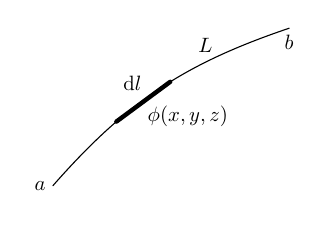
\begin{tikzpicture}[
    line cap=round,
    every node/.style={scale=.75}
]
  \draw 
    (0,0) 
    node[left] {$a$} 
    to[bend left=15] 
    coordinate[pos=.3] (a) 
    coordinate[pos=.55] (b) 
    node[above=1pt,pos=.7] {$L$} 
    (3,2) 
    node[below] {$b$}
  ;
  \draw[ultra thick] (a) 
    -- node[pos=.3,above=5pt] {$\d l$} 
    node[below right=-2pt] {$\phi(x,y,z)$}
    (b)
  ;
\end{tikzpicture}

\end{document}